\documentclass[a4paper, 12pt]{extarticle}

% Поля
%--------------------------------------
\usepackage{geometry}
\geometry{a4paper,tmargin=2cm,bmargin=2cm,lmargin=3cm,rmargin=1cm}
%--------------------------------------


%Russian-specific packages
%--------------------------------------
\usepackage[T2A]{fontenc}
\usepackage[utf8]{inputenc} 
\usepackage[english, main=russian]{babel}
%--------------------------------------

\usepackage{textcomp}

% Красная строка
%--------------------------------------
\usepackage{indentfirst}               
%--------------------------------------             


%Graphics
%--------------------------------------
\usepackage{graphicx}
\graphicspath{ {./images/} }
\usepackage{wrapfig}
\usepackage{minted}
%--------------------------------------

% Полуторный интервал
%--------------------------------------
\linespread{1.3}                    
%--------------------------------------

%Выравнивание и переносы
%--------------------------------------
% Избавляемся от переполнений
\sloppy
% Запрещаем разрыв страницы после первой строки абзаца
\clubpenalty=10000
% Запрещаем разрыв страницы после последней строки абзаца
\widowpenalty=10000
%--------------------------------------

%Списки
\usepackage{enumitem}

%Подписи
\usepackage{caption} 

%Гиперссылки
\usepackage{hyperref}

\hypersetup {
	unicode=true
}

%Рисунки
%--------------------------------------
\DeclareCaptionLabelSeparator*{emdash}{~--- }
\captionsetup[figure]{labelsep=emdash,font=onehalfspacing,position=bottom}
%--------------------------------------

\usepackage{tempora}
\usepackage{amsmath}
\usepackage{color}
\usepackage{listings}
\lstset{
  belowcaptionskip=1\baselineskip,
  breaklines=true,
  frame=L,
  xleftmargin=\parindent,
  language=Python,
  showstringspaces=false,
  basicstyle=\footnotesize\ttfamily,
  keywordstyle=\bfseries\color{blue},
  commentstyle=\itshape\color{purple},
  identifierstyle=\color{black},
  stringstyle=\color{red},
}

%--------------------------------------
%			НАЧАЛО ДОКУМЕНТА
%--------------------------------------

\begin{document}

%--------------------------------------
%			ТИТУЛЬНЫЙ ЛИСТ
%--------------------------------------
\begin{titlepage}
\thispagestyle{empty}
\newpage


%Шапка титульного листа
%--------------------------------------
\vspace*{-30 pt}
\hspace{-65pt}
\begin{minipage}{0.3\textwidth}
\hspace*{-20pt}\centering

\includegraphics[width=60pt]{emblem}
\end{minipage}
\begin{minipage}{0.67\textwidth}\small \textbf{
\vspace*{-0.7ex}
\hspace*{-6pt}\centerline{Министерство науки и высшего образования Российской Федерации}
\vspace*{-0.7ex}
\centerline{Федеральное государственное бюджетное образовательное учреждение }
\vspace*{-0.7ex}
\centerline{высшего образования}
\vspace*{-0.7ex}
\centerline{<<Московский государственный технический университет}
\vspace*{-0.7ex}
\centerline{имени Н.Э. Баумана}
\vspace*{-0.7ex}
\centerline{(национальный исследовательский университет)>>}
\vspace*{-0.7ex}
\centerline{(МГТУ им. Н.Э. Баумана)}}
\end{minipage}
%--------------------------------------

\vspace{10pt}
\hspace{-35pt} \noindent \small ФАКУЛЬТЕТ\hspace{80pt} <<Информатика и системы управления>>

\vspace*{-16pt}
\hspace{47pt}\rule{0.83\textwidth}{0.4pt}

\vspace{0.5ex}
\hspace{-35pt} \noindent \small КАФЕДРА\hspace{50pt} <<Теоретическая информатика и компьютерные технологии>>

\vspace*{-16pt}
\hspace{30pt}\rule{0.866\textwidth}{0.4pt}
  
\vspace{6em}

\begin{center}
\Large {\bf Лабораторная работа №5} \\ 
\large {\bf по курсу <<Языки и методы программирования>>} \\ 
\large «Монады в языке Java» \\
\large <<Вариант 31>>
\end{center}\normalsize

\vspace{15em}


\begin{flushright}
  {Студент группы ИУ9-21Б: Пенкин А. Д.\hspace*{15pt} \\
  \vspace{2ex}
  Преподаватель: Посевин Д. П.\hspace*{15pt}}
\end{flushright}

\bigskip

\vfill
 \vspace{7em}

\begin{center}
\textsl{Москва 2023}
\end{center}
\end{titlepage}
%--------------------------------------
%		КОНЕЦ ТИТУЛЬНОГО ЛИСТА
%--------------------------------------

\renewcommand{\ttdefault}{pcr}

\setlength{\tabcolsep}{3pt}
\newpage
\setcounter{page}{2}

\section{Цель}\label{Sect::task}
\par
Приобретение навыков использования монад Optional и Stream в программах на языке Java. 
\section{Условие}
\par
Во время выполнения лабораторной работы требуется разработать на языке Java Булевскую матрицу размером m × n, где 1 <= m, n <=
8, с операциями:
\par
1. порождение потока сумм элементов строк по модулю 2 (т.е., исключающее ИЛИ);
\par
2. поиск строки, в которой единиц больше, чем во всех остальных строках вместе взятых. Элементы матрицы должны быть представлены битами в числе типа long. 
\par
Проверить работу первой операции нужно путём подсчёта количеств вхождений каждого из присутствующих в последовательности чисел.
\section{Код решения}
1. Test.java
\begin{minted}{java}
public class Test {
    public static void main(String[] args) {
        MatrixBool A = new MatrixBool(new int[][]{
                {1, 1, 1, 0},
                {1, 0, 1, 0},
                {0, 1, 1, 1},
                {0, 1, 1, 0},
                {0, 0, 0, 1}});
        MatrixBool B = new MatrixBool(new int[][]{
                {1, 1, 1, 1, 1, 1, 0, 1},
                {0, 0, 0, 1, 0, 0, 0, 1},
                {0, 0, 0, 0, 0, 0, 1, 0},
                {0, 0, 1, 0, 0, 0, 0, 0}});

        System.out.println("Создадим матрицу 1:");
        A.printMatrix();
        System.out.println("");
        System.out.println("Создадим матрицу 2:");
        B.printMatrix();
        System.out.println("");

        System.out.println("Выведем через поток исключающее или");
        System.out.println("для каждой из строк матрицы 1 и 2:");
        System.out.print("**");
        A.xorStream().forEach(x -> System.out.print(" " + x + " "));
        System.out.println("**");
        System.out.print("**");
        B.xorStream().forEach(x -> System.out.print(" " + x + " "));
        System.out.println("**");

        System.out.println("Посчитаем количество \"1\" и \"0\" в этих потоках:");
        System.out.print("\"1\" - " + A.xorStream().filter(x -> x == 1).count());
        System.out.println("; \"0\" - " + A.xorStream().filter(x -> x == 0).count());
        System.out.print("\"1\" - " + B.xorStream().filter(x -> x == 1).count());
        System.out.println("; \"0\" - " + B.xorStream().filter(x -> x == 0).count() + "\n");

        System.out.println("Найдём строку, матрицы 1, в которой \"1\"");
        System.out.println("больше чем в остальных строках вместе взятых:");
        if (A.getBestString().isPresent()) {
            System.out.println(A.getBestString().get().getString() + "\n");
        }
        else {
            System.out.println("такой строки не существует.\n");
        }

        System.out.println("Найдём строку, матрицы 2, в которой \"1\"");
        System.out.println("больше чем в остальных строках вместе взятых:");
        if (B.getBestString().isPresent()) {
            System.out.println(B.getBestString().get().getString() + "\n");
        }
        else {
            System.out.println("такой строки не существует.");
        }
    }
}
\end{minted}
2. MatrixBool.java
\begin{minted}{java}
import java.util.Arrays;
import java.util.*;
import java.util.stream.Stream;

public class MatrixBool {
    private ArrayList<StringMatrix> A;
    long n;
    public MatrixBool(int[][] A1) {
        A = new ArrayList<>(1);
        Arrays.stream(A1)
                .map(x -> new StringMatrix(x))
                .forEach(x -> A.add(x));
        n = A.stream()
                .map(x -> x.getSumBinary())
                .reduce((x, y) -> x + y).get();
    }

    public StringMatrix getStringMatrix(int i){
        return A.get(i);
    }

    public long getN() {
        return n;
    }

    public void printMatrix(){
        A.stream().map(x -> x.getString())
                .map(x -> x.split(""))
                .forEach(x -> {
                    Arrays.stream(x)
                            .forEach(y -> System.out.print(y + " "));
                    System.out.println("");
                });
    }

    public Stream<Long> xorStream() {
        ArrayList<Long> result = new ArrayList<>();
        A.stream()
                .map(x -> x.getSumBinary() % 2)
                .forEach(x -> result.add(x));
        return result.stream();
    }

    public Optional<StringMatrix> getBestString() {
        Optional<StringMatrix> result = Optional.empty();
        Optional<StringMatrix> tmp = A
                .stream()
                .filter(x -> x.getSumBinary() > n - x.getSumBinary())
                .findFirst();
        if (tmp.isPresent()) {
            result = Optional.ofNullable(tmp.get());
        }
        return result;
    }
}
\end{minted}
3. StringMatrix.java
\begin{minted}{java}
import java.util.Arrays;

public class StringMatrix {
    private long str, sumBinary;
    int count;
    public StringMatrix(int[] a) {
        str = 0;
        Arrays.stream(a).forEach(y-> {
            str = (str << 1) + y;
            sumBinary += y;});
        count = a.length;
    }

    public long getSumBinary() {
        return sumBinary;
    }

    public long getStr() {
        return str;
    }
    public String getString(){
        String a = Long.toBinaryString(str);
        if (a.length() < count){
            a = "0".repeat(count - a.length()) + a;
        }
        return a;
    }
}
\end{minted}

\section{Результаты работы программы}
\begin{figure}[H]
    \centering
    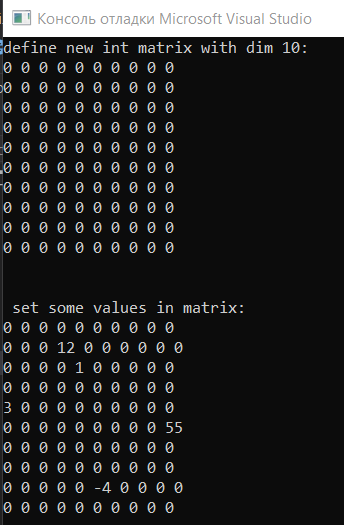
\includegraphics[width=170pt]{Test.png}
    \caption{создание матриц и их вывод}
    \label{fig:my_label}
\end{figure}

\begin{figure}[H]
    \centering
    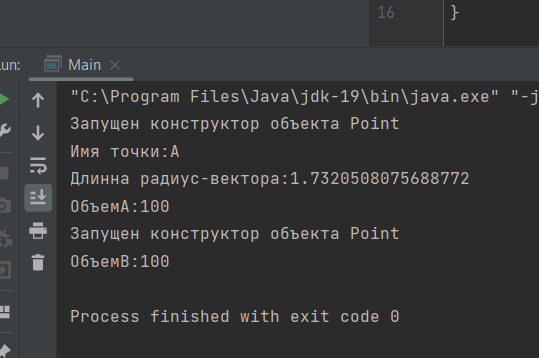
\includegraphics[width=400pt]{Test1.png}
    \caption{работа потока исключающего или}
    \label{fig:my_label}
\end{figure}

\begin{figure}[H]
    \centering
    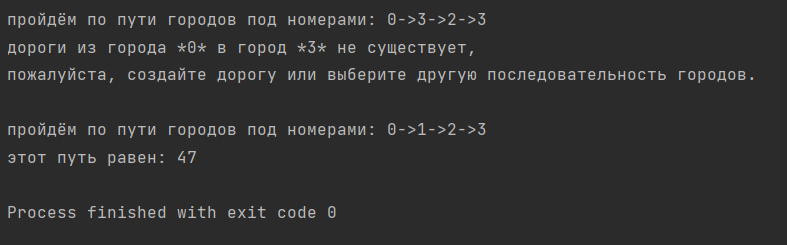
\includegraphics[width=400pt]{Test2.png}
    \caption{поиск строки с наибольшим количеством единиц}
    \label{fig:my_label}
\end{figure}


\end{document}